\documentclass[10pt,twocolumn]{article}
\usepackage[margin=0.75in]{geometry}
\usepackage{booktabs}
\usepackage{graphicx}
\usepackage{tikz}
\usetikzlibrary{arrows.meta,positioning}
\usepackage[hidelinks]{hyperref}
\usepackage{caption}
\usepackage{enumitem}
\usepackage{url}
\usepackage{amsmath}
\setlength{\columnsep}{0.22in}
\setlength{\emergencystretch}{2em}

\title{DRC Explain: Verification-Grounded LLM Explanations for SKY130 Layout Checks}
\author{Rana Shamoun and Giovanni Cascone\\
San Jose State University -- CMPE 258 Deep Learning}
\date{December 2026}

\begin{document}
\maketitle

\begin{abstract}
We present DRC Explain, a bounded language-model agent for explaining selected SKY130
layout design-rule checks. The system combines rule retrieval, layout inspection,
KLayout DRC execution, and deterministic verification of structured model claims.
It does not edit layouts or replace physical verification: accepted PASS/FAIL verdicts
apply only to the rule IDs selected by the model. We evaluate coordinate-only (A),
retrieval-only (B), and tool-grounded (C) conditions on a frozen 168-record grid for
Qwen3 8B, GPT-4o, and Gemini 3.5 Flash-Lite. In C, GPT-4o and Qwen3 score 50/50
benchmark verdicts, while Gemini scores 46/50; execution errors are 0, 5, and 9
respectively. We also add a separate 24-layout held-out set and preserve fixed
denominators. The results are preliminary and not foundry signoff.
\end{abstract}

\section{Introduction}
DRC engines identify geometric violations, but users need to determine which rules
apply and interpret evidence in a focused engineering question. A language model may
hallucinate thresholds or fabricate measurements. DRC Explain therefore keeps
KLayout as the source of geometric truth and constrains model-generated explanations
to structured, verifier-accepted claims.

The project addresses three questions: (1) whether rule retrieval improves model
predictions, (2) whether tool-grounded verification improves end-to-end reliability,
and (3) how execution failures should be reported. The prototype supports eight
curated ordinary metal1/metal2 width and spacing rules and minimum/corner enclosure
for square 0.15~\textmu m vias. It is not a full-chip signoff system.

\section{System}
\begin{figure}[t]
\centering
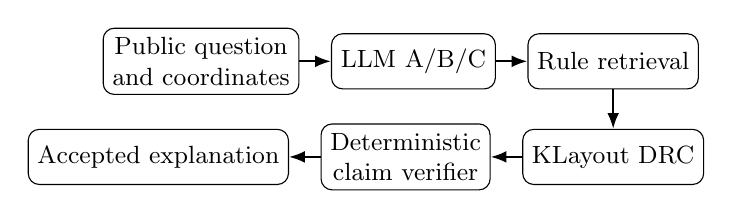
\begin{tikzpicture}[node distance=5mm and 4mm,
 block/.style={draw,rounded corners,align=center,font=\small,minimum height=7mm},
 arrow/.style={-{Latex[length=2mm]},thick}]
\node[block] (q) {Public question\\and coordinates};
\node[block,right=of q] (m) {LLM A/B/C};
\node[block,right=of m] (r) {Rule retrieval};
\node[block,below=of r] (d) {KLayout DRC};
\node[block,left=of d] (v) {Deterministic\\claim verifier};
\node[block,left=of v] (e) {Accepted explanation};
\draw[arrow] (q)--(m);
\draw[arrow] (m)--(r);
\draw[arrow] (r)--(d);
\draw[arrow] (d)--(v);
\draw[arrow] (v)--(e);
\end{tikzpicture}
\caption{DRC Explain workflow. The model interprets and proposes; tools and the verifier remain authoritative.}
\label{fig:system}
\end{figure}

Condition A supplies only the question and layout coordinates. Condition B adds
supported-rule retrieval. Condition C permits bounded rule retrieval, layout
inspection, KLayout checks, and structured finalization.

The agent submits \texttt{selections} and per-rule \texttt{claims}. The verifier checks
selected rule IDs, claim completeness, PASS/FAIL consistency, limits, and available
edge-pair measurements against evidence from the unchanged public GDS. Unsupported
requests receive REFUSE; runtime failures and exhausted turn budgets produce ERROR.
ERROR is not a geometric FAIL and is not a domain refusal.

The agent does not modify GDS layouts and does not call Magic or OpenROAD. It is a
read-only explanation and verification agent. KLayout executes the full pinned
upstream SKY130 deck and filters the output to selected checks; the final text is deterministically rendered
from accepted facts rather than unrestricted free-form prose.

\section{Benchmarks and Held-Out Data}
The development/public benchmark contains 50 labeled layouts and six unsupported
scope probes. It includes near-boundary spacing, pass/fail pairs, competing rules,
and conditional via enclosure. Six development layouts were also used for
demonstrations and are disclosed separately.

The 24-layout held-out set is excluded from the original public/evaluator workflow.
It contains six near-boundary cases, six pass/fail-pair members, six competing-rule
layouts, and six conditional-enclosure layouts, plus three refusal probes. Layout
hashes, construction intent, private labels, and native-RDB reports are retained
for verification. The held-out generator and the original benchmark use the same
geometry builder and KLayout engine, so this set strengthens implementation
separation but is not an independent oracle implementation.

\section{Scoring Protocol}
For the 50-layout benchmark, accuracy is
\[
\mathrm{Accuracy}=\frac{\#\{\text{correct accepted verdicts}\}}{50}.
\]
Every execution ERROR is counted incorrect. The 56-record total includes six probes,
for which refusal correctness is reported separately. An accepted-output count
describes the number of records that produced a verifier-accepted or structurally
valid answer and must not replace fixed-denominator accuracy.

The repeated held-out protocol uses the fixed 24-layout denominator. For each
repetition, we report accuracy and preserve each original ERROR record.
Retries are placed in separate run directories and never replace the original result.

\section{Experimental Results}
\begin{table}[t]
\centering
\caption{Frozen 168-record grids: 50 benchmark verdicts plus six probes in each condition.}
\label{tab:results}
\small
\begin{tabular}{lrrrr}
\toprule
Model & A & B & C & ERROR \\
\midrule
Qwen3 8B & 23/50 & 29/50 & 50/50 & 5 \\
GPT-4o & 29/50 & 27/50 & 50/50 & 0 \\
Gemini & 41/50 & 43/50 & 46/50 & 9 \\
\bottomrule
\end{tabular}
\end{table}

Table~\ref{tab:results} reports all three grids once under matching public inputs,
prompt text, implementation hashes, conditions, and one repetition. GPT-4o completed
all 168 records. Qwen completed all records with three B and two C errors, while its
C benchmark verdict accuracy remained 50/50. Gemini had three A HTTP 503s, two B
turn-budget failures, and four C protocol failures. Gemini's C accuracy is 46/50,
not 46/37 or another conditional accepted-output denominator.

The main result is that tool-grounded C is strongest in this exposed comparison,
but the result does not isolate the causal effect of KLayout because C combines
retrieval, tools, verification, and rendering. It also does not establish reliability
for Gemini or generalization to unseen layouts.

\subsection{Held-Out Stability for Qwen3}
Three separate condition-C repetitions were completed on the 24-layout held-out set.
Each repetition scored 24/24 benchmark verdicts, 3/3 unsupported-scope refusals,
and 0 execution ERROR records. Selection recall was 1.000 and refusal correctness
was 1.000 in every repetition. The mean accuracy was 100\% with a 100--100\% range.
This provides repeated held-out stability evidence for local Qwen3 C on this dataset
and does not establish foundry signoff.

\subsection{Three-Model Held-Out Comparison}
Matching held-out condition-C repetitions were then completed for GPT-4o and
Gemini 3.5 Flash-Lite. GPT-4o scored 24/24 in each repetition with 0 execution
errors. Gemini scored 20/24, 14/24, and 15/24 in the historical no-503-retry run.
The original Gemini run had 22 HTTP 503 errors and one protocol error. After adding
up to five bounded HTTP 503 retries, a separate run scored 22/24, 21/24, and 19/24
with 13 ERROR records across 81 records. Its probe refusals were 1/3, 2/3, and 3/3.
Qwen3, GPT-4o, and the original Gemini run had 3/3 refusals in every repetition.
Changed code and provider conditions prevent a causal attribution to retries.
GPT-4o repeated cost was
\$0.350, \$0.346, and \$0.355 according to the application estimate ledger.

A subsequent eight-retry Gemini run scored 18/24, 0/24, and 0/24, with 0/3
probe refusals in each repetition and 63/81 ERROR records, all HTTP 429 quota
failures. The free-tier daily request quota was exhausted; this run measures
quota-limited execution rather than Gemini's answer quality. It is not pooled
with the earlier runs.

\section{Validity and Limitations}
\begin{itemize}[leftmargin=*]
\item The 50-layout and 24-layout sets are small and curated.
\item The development benchmark was exposed during debugging and demonstrations.
\item The oracle and implementation use the same KLayout engine and pinned deck.
\item The project does not evaluate an external standard open-source SKY130/OpenROAD
suite and has no independent physical signoff oracle.
\item One repetition on the frozen grids provides no run-to-run uncertainty.
\item C verifies only selected rules; PASS is not full-chip signoff.
\item The original upstream deck scope is incomplete for a fabrication PDK.
\end{itemize}

\section{Implementation and Reproducibility}
The repository includes the agent, provider adapters, KLayout runner, structured
claim verifier, experiment runner, synthetic layout generator, held-out verifier,
automated tests, UI, progress report, and demo guide. The code records prompt and
implementation hashes, public dataset paths, provider metadata, usage, latency,
tool calls, verification status, and original ERROR messages. Credentials are kept
outside source control.

The repository is at
\url{https://github.com/RanaShamoun/llm-sky130-drc-agent}.
On November 25, 2026, \texttt{run.py check} passed 117 tests with one platform-specific skip,
and the held-out 24/24 construction/oracle verification had no mismatches.

\section{Conclusion and Next Evaluation}
The matching held-out condition-C study is complete for Qwen3, GPT-4o, and Gemini.
Report fixed-denominator held-out accuracy, accepted-output counts, per-repetition
ranges, and execution-error rates. GPT-4o and Qwen3 remained 24/24 in all repetitions,
while separate Gemini runs showed substantial service and quota errors despite
bounded retries. External layout suites or an independent physical oracle
would still be required for signoff-level claims.

\section*{Resources}
\url{https://github.com/RanaShamoun/llm-sky130-drc-agent}
\end{document}
